\documentclass[tikz]{standalone}

%: === FONT === (((
\usepackage{fontspec}
\setmainfont[
  BoldFont       = bodonibi,
	ItalicFont     = Century modern italic2.ttf,
	BoldItalicFont = bodonibi,
	SmallCapsFont  = lmromancaps10-regular.otf
]{Century_modern.ttf}
\DeclareSymbolFont{italics}{\encodingdefault}{\rmdefault}{m}{it}
\DeclareSymbolFontAlphabet{\mathit}{italics}
\ExplSyntaxOn
\int_step_inline:nnnn { `A } { 1 } { `Z }
 {  \exp_args:Nf \DeclareMathSymbol{\char_generate:nn{#1}{11}}{\mathalpha}{italics}{#1} }
\int_step_inline:nnnn { `a } { 1 } { `z } {  \exp_args:Nf \DeclareMathSymbol{\char_generate:nn{#1}{11}}{\mathalpha}{italics}{#1}}
\ExplSyntaxOff
% )))

\begin{document}

\begin{tikzpicture}[>=latex]

	\node [opacity=0,rotate=0.2] at (2.15,1.91) {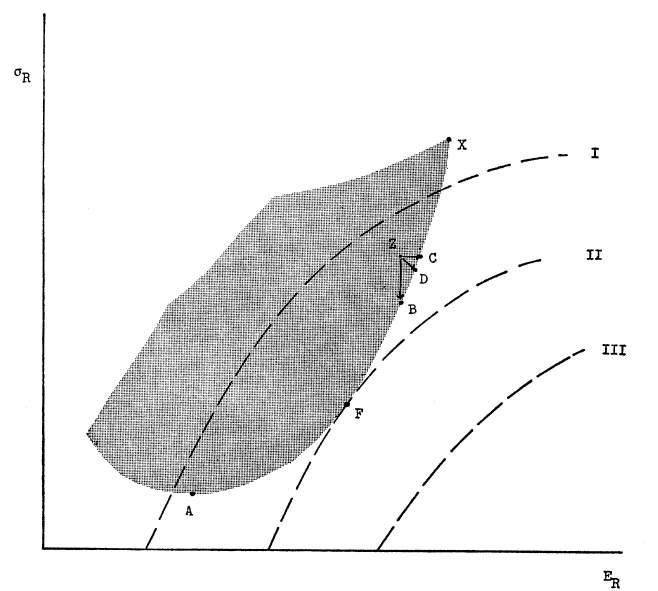
\includegraphics[width= 5cm]{2.png}};
	% \draw (0,0) grid (4,4);
	\draw (0,0) -- (4,0);
	\draw (0,0) -- (0,4);
	\fill (3.35,1) circle (1pt);
	\draw [->] (3.35,1) --++ (0.5,-0.5);

\end{tikzpicture}

\end{document}
